% ----------------------------------------------------------
% Capítulo 2
% ----------------------------------------------------------
\chapter{Estratégia de Deploy e Resiliência}
\label{chap:deploy-resiliencia}

Esta seção detalha as estratégias propostas para garantir entregas de software frequentes, confiáveis e com baixo risco para o Sistema VOEBEM, abordando o pipeline de CI/CD, a metodologia de deploy em produção e o plano de rollback.

\section{Pipeline de CI/CD (Integração Contínua / Entrega Contínua)}
\label{sec:cicd}

Propõe-se um pipeline de CI/CD robusto para automatizar o processo de build, teste e deploy dos diferentes containers (microsserviços, frontend) do sistema, conforme ilustrado abaixo.

\subsection{Ferramentas Propostas}
\label{subsec:cicd-ferramentas}
\begin{itemize}
    \item \textbf{Controle de Versão:} Git (com repositórios hospedados no GitLab ou GitHub).
    \item \textbf{Servidor de CI/CD:} GitLab CI/CD ou GitHub Actions (integrados à plataforma de repositórios).
    \item \textbf{Containerização:} Docker (para empacotar as aplicações e suas dependências).
    \item \textbf{Registro de Container:} Docker Hub, GitLab Container Registry, AWS ECR ou similar.
    \item \textbf{Orquestração de Containers:} Kubernetes (gerenciado na nuvem, Exemplo: AWS EKS, Google GKE, Azure AKS).
    \item \textbf{Ferramentas de Teste:} JUnit (para Java/API Reservas), PyTest (para Python/API Voos), Jest/Cypress (para Frontend React).
    \item \textbf{Análise de Código (Opcional):} SonarQube (para análise estática de segurança e qualidade).
\end{itemize}

\subsection{Fluxo do Pipeline}
\label{subsec:cicd-fluxo}
O diagrama abaixo ilustra as etapas sequenciais e pontos de decisão do pipeline, desde o commit do código até o deploy em produção, incluindo validações intermediárias.

\begin{figure}[htbp]
    \centering
    % Ajustando largura para consistência com Cap. 3
    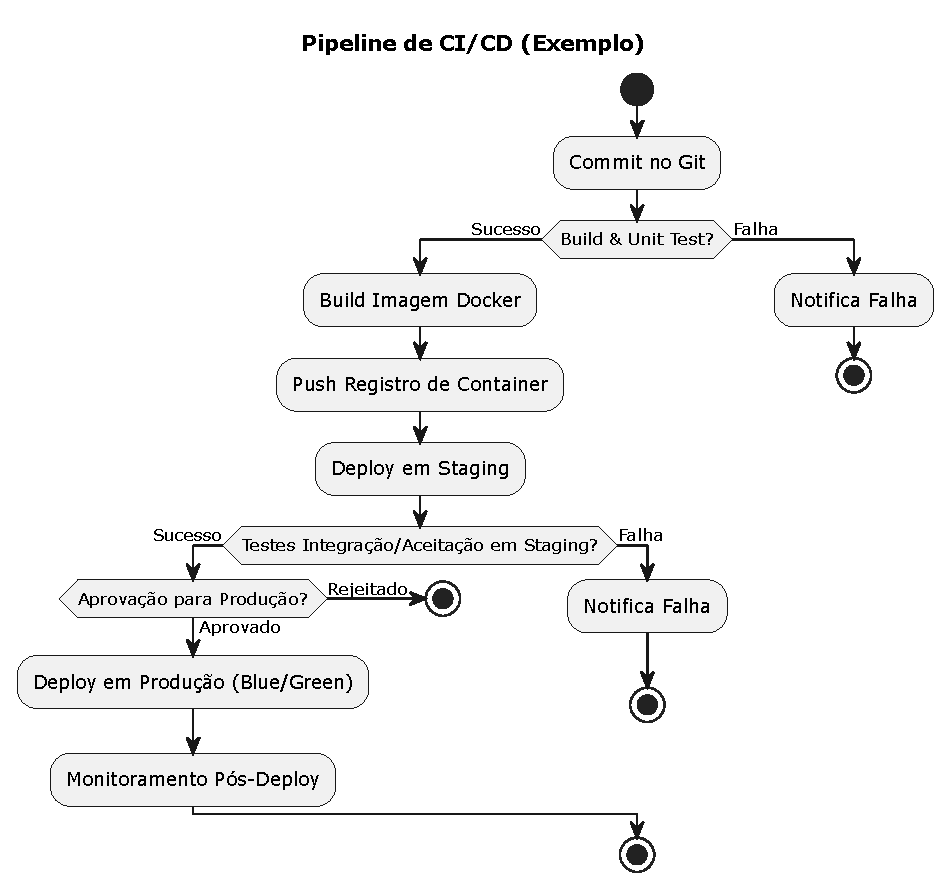
\includegraphics[width=0.8\textwidth]{../assets/diagrama-cicd.pdf}
    \caption{Diagrama do Pipeline de CI/CD}
    \label{fig:diagrama-cicd}
\end{figure}

\subsection{Etapas Detalhadas}
\label{subsec:cicd-etapas}
\begin{enumerate}
    \item \textbf{Commit \& Trigger:} Desenvolvedor envia código, iniciando o pipeline.
    \item \textbf{Build \& Unit Test:} Compilação e testes unitários. Falhas interrompem o pipeline.
    \item \textbf{Code Scan (Opcional):} Análise estática de código.
    \item \textbf{Build da Imagem Docker:} Criação da imagem da aplicação.
    \item \textbf{Push para Registro:} Envio da imagem para o registro.
    \item \textbf{Deploy em Staging:} Implantação em ambiente de homologação.
    \item \textbf{Testes de Integração/Aceitação:} Validação funcional e de integração em Staging. Falhas interrompem o pipeline.
    \item \textbf{Aprovação (Manual/Automática):} Ponto de controle antes da produção.
    \item \textbf{Deploy em Produção:} Implantação em produção usando a estratégia Blue/Green.
    \item \textbf{Monitoramento Pós-Deploy:} Observação ativa da nova versão em produção.
\end{enumerate}

\section{Estratégia de Deploy}
\label{sec:estrategia-deploy}

Considerando a criticidade do sistema e a necessidade de minimizar riscos e downtime, a estratégia de deploy recomendada é \textbf{Blue/Green Deployment}, cujo fluxo é apresentado no diagrama a seguir.

\subsection{Justificativa}
\label{subsec:deploy-justificativa}
\begin{itemize}
    \item \textbf{Zero Downtime:} Transição suave de tráfego.
    \item \textbf{Testes em Produção Isolados:} Validação da nova versão sem impacto no usuário.
    \item \textbf{Rollback Instantâneo:} Reversão rápida em caso de problemas.
    \item \textbf{Simplicidade Conceitual:} Fluxo claro para deploy e rollback.
\end{itemize}

\subsection{Funcionamento (Ilustrado no Diagrama)}
\label{subsec:deploy-funcionamento}

\begin{figure}[htbp]
    \centering
    % Ajustando largura para consistência com Cap. 3
    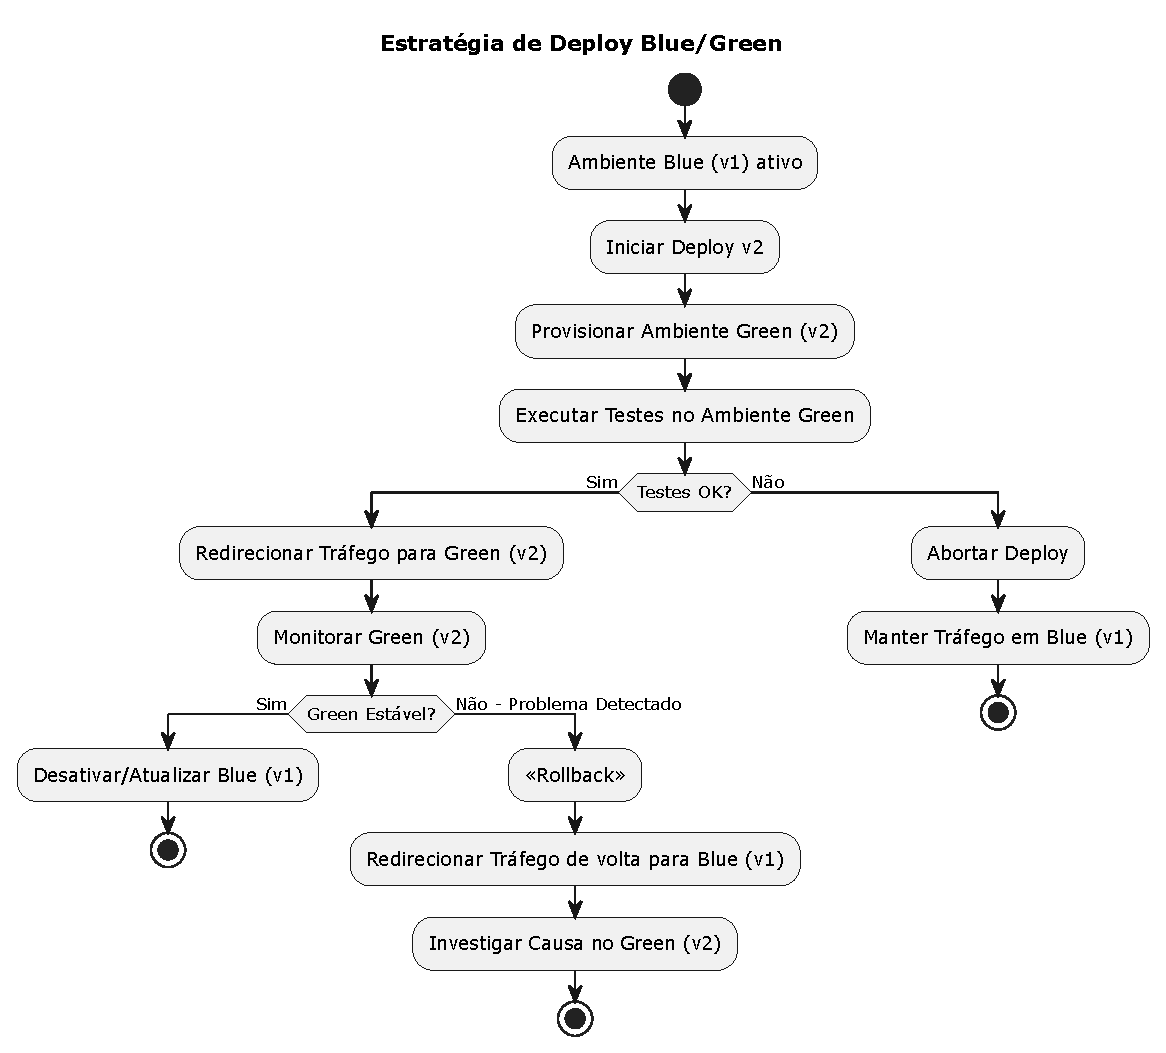
\includegraphics[width=0.8\textwidth]{../assets/diagrama-bluegreen.pdf}
    \caption{Diagrama da Estratégia Blue/Green}
    \label{fig:diagrama-bluegreen}
\end{figure}

\begin{enumerate}
    \item \textbf{Ambiente Blue Ativo:} Versão atual (v1) recebe o tráfego.
    \item \textbf{Provisionamento Green:} Nova versão (v2) é implantada em um ambiente idêntico (Green).
    \item \textbf{Testes no Green:} Validação da v2 no ambiente Green isolado.
    \item \textbf{Switch de Tráfego:} Se os testes passarem, o tráfego é direcionado para o ambiente Green (v2).
    \item \textbf{Monitoramento do Green:} A v2 é monitorada em produção.
    \item \textbf{Estabilização ou Rollback:} Se a v2 estiver estável, o ambiente Blue (v1) é desativado. Se problemas críticos forem detectados, o tráfego é revertido imediatamente para o Blue (v1) (Rollback).
    \item \textbf{Desativação do Blue:} Após confirmação da estabilidade do Green, o ambiente Blue é liberado.
\end{enumerate}

\subsection{Benefícios para VOEBEM}
\label{subsec:deploy-beneficios}
Essa abordagem minimiza o risco de impacto ao usuário durante atualizações e permite reversões imediatas caso surjam problemas inesperados, garantindo assim a continuidade das operações críticas de reserva e a confiança do cliente.

\section{Estratégia de Rollback}
\label{sec:estrategia-rollback}

A estratégia de rollback é uma parte intrínseca do fluxo Blue/Green, como visualizado no diagrama anterior.

\subsection{Processo de Rollback (Detalhado)}
\label{subsec:rollback-processo}
\begin{enumerate}
    \item \textbf{Detecção de Problema:} Identificação de falha crítica na versão Green (v2) ativa, via monitoramento ou alertas.
    \item \textbf{Acionamento:} Manual pela equipe SRE/Operações ou automático por violação de SLOs.
    \item \textbf{Redirecionamento de Tráfego:} Reconfiguração do Load Balancer/Roteador para enviar 100% do tráfego de volta ao ambiente Blue (v1), que contém a versão estável anterior. Esta é a ação principal e imediata do rollback.
    \item \textbf{Análise de Causa Raiz:} Investigação do problema no ambiente Green (v2), agora isolado.
    \item \textbf{Correção e Novo Deploy:} Após correção, o ciclo de deploy pode ser reiniciado.
\end{enumerate}

\subsection{Garantias}
\label{subsec:rollback-garantias}
\begin{itemize}
    \item \textbf{Velocidade:} MTTR minimizado pela rapidez do redirecionamento.
    \item \textbf{Segurança:} Versão estável anterior sempre disponível.
    \item \textbf{Consistência:} Processo claro e passível de automação.
\end{itemize}

% --- Final do Arquivo ---
